% !TEX root = ../paper.tex
% chapter3

\section{Project Management Problem}
%

\subsection{Project Plan}
%

The core of project management problem is work package scheduling and resource
allocation.
Figure \ref{fig:sample} is a Gantt chart of typical software project management, which
illustrates work package arrangement of a real industry software engineering.
Generally, all the important phases in software engineering, such as project
planning, requirements analysis, design, development, testing, deployment etc., are inseparable from the allocation of work packages.  These work
packages have a mutually restrictive relationship. Some work packages must be
started when other work packages are completed. For instance, the analysis of
software requirements is often to take place after the completion of project planning
while some work packages can be done at the same time, and there is no
impact on each other, such as software development and software testing can
often be synchronized. The goal of project manager is using the shortest possible time
to complete all work packages within the software project duration.

% figure 2
%\vspace{-6mm}
\begin{figure}[!ht]
  \centering
%  \vspace{-6mm}
  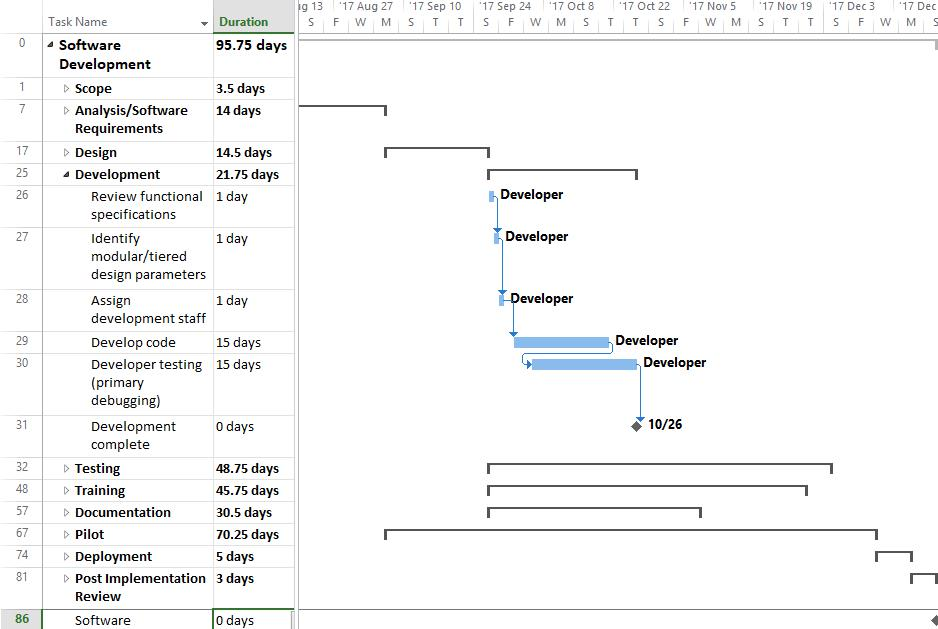
\includegraphics[width=0.9\textwidth]{figures/pm_sample.jpg}
  \vspace{-2mm}
  \caption{Software Project Plan in a Microsoft Project File (.mpp)}
  \label{fig:sample}
  \vspace{-2mm}
\end{figure}


\begin{figure}[!ht]
  \centering
  \vspace{-3mm}
  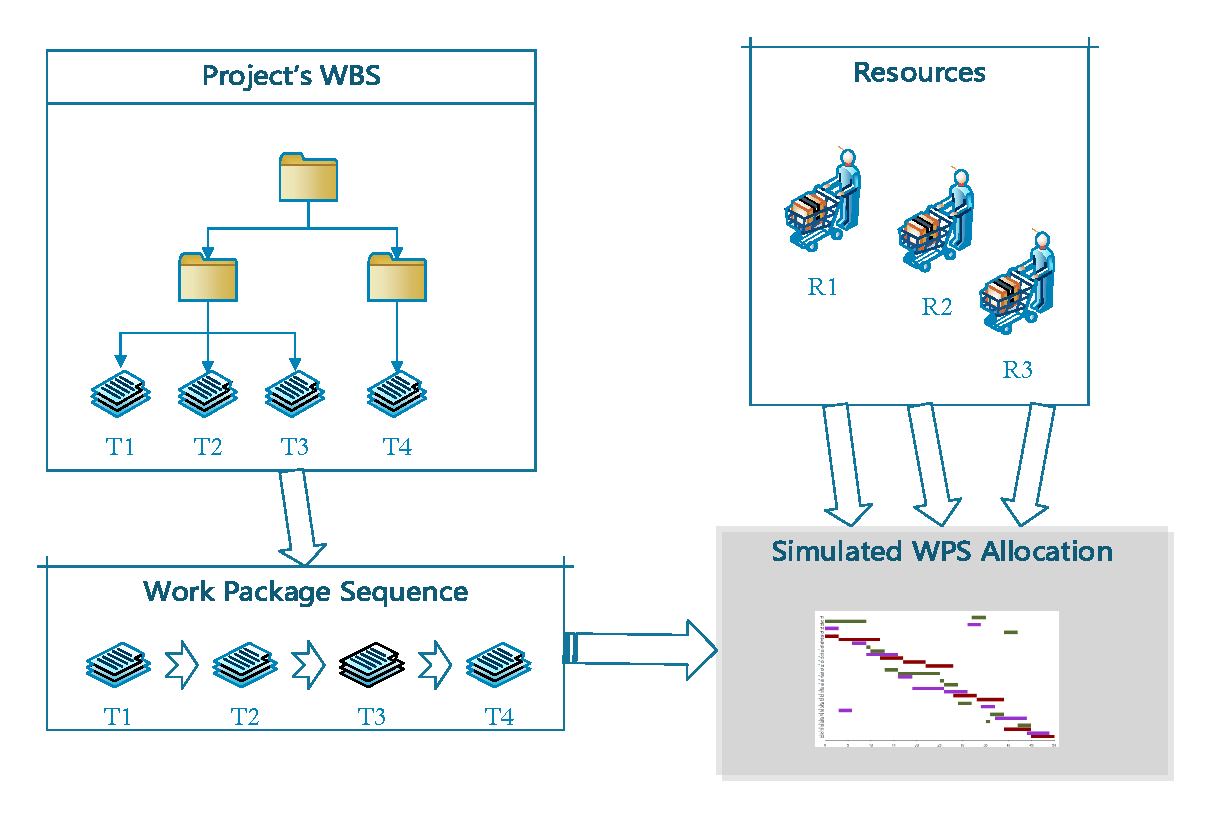
\includegraphics[width=0.8\textwidth]{figures/simu.pdf}
  \vspace{-5mm}
  \caption{Project Plan of Software Development}
  \label{fig:simu}
\vspace{-5mm}
\end{figure}


 In the process of project management, the work packages in the project are
 allocated by simulation. See figure \ref{fig:simu}, Firstly, the whole project
 is decomposed into several work packages by \emph{work breakdown structure},
 and those work packages are arranged into a corresponding \emph{work package
   sequence}. Secondly, according to the dependencies of the work packages and
 the restriction of resource, each kinds of resources is allocated to the
 corresponding work package by \emph{first-come-first-served}
 algorithm. Finally, the project's overall duration is yielded from the simulation.



\subsection{Definition and Assumptions}
%
The goal of this paper is to find an optimal solution or near optimal
solution for the project management problem described as follows:


\emph{
  For a software project with $N$ work packages and $M$ kinds of resources,
  there is a directed acyclic dependencies between these work packages, and each
  resource can only be assigned to the specified work package.  It is necessary
  to arrange the order of the work package reasonably and make the overall
  construction duration as short as possible under the condition of satisfying
  the work package dependency and the resource allocation restriction.
}

%
There are three assumptions for our project management problem.

Assumption I: The software project plan can be decomposed into a set of
work packages containing $N$ elements $T = \{t_1, t_2, ..., t_N \}$.
Each work package in set $T$ is indivisible (i.e., The work package cannot be
split to other work package in the schedule), the set of work packages have a
pre-estimated workload, the composition of the workload is the collection
$E = \{e _1, e_2, ..., e_N \}$. The function $TE: T \rightarrow E$,
the mean of this function is that for a given work package $t_i$, produces an
estimated workload $e_i = TE(t_i)$ for a work package $t_i$, where $e_i$ is the
estimated workload of $t_i$.


Assumption II: The work packages in the software project  can be
processed with $M$ kinds of resources, which constitute a resource set
$R = \{r_1, r_2, ..., r_M \}$, for each project's work package set $T$ and the
resource set $R$, There exists a function $TR: T \times R \rightarrow \{0, 1\}$,
for the given work package $t_i$ and the resource $r_j$, $TR(t_i, r_j) = 1$
means the resource $r_j$ can be allocated to the work package $t_i$, while
$TR(t_i, r_j) = 0$ means cannot.


Assumption III: All work packages in the set $T$ of the software project
plan have dependencies. These dependencies form a set
$Dep= \{t_i \rightarrow t_j \mid t_i, t_j \in T, t_j \text{ depends on } t_i\}$.
As the assumption of this paper, $t_i \rightarrow t_j$ means that $t_j$ depends
on $t_i$, that is the work package $t_j$ must be arranged after the work
package $t_i$, and satisfy the formula $t_j.start \leq t_i.end$ (where $t.start$
and $t.end$ respectively indicate the start time and the end time of the work
package $t$).  And assume that there is no direct or indirect "loop" dependency
between work packages.


  \vspace{-2mm}


\subsection{The Objective of Problem}
%
The objective of project management is to find an optimal work package sequence
under the three assumptions above.
The notation of work package sequence(WPS) is as follows:
\begin{equation}
\vspace{-2mm}
  S = \{
  (t_{p_1}, r_{q_1}) ... \rightarrow (t_{p_j}, r_{q_j}) \rightarrow ... (t_{p_N}, r_{q_N})
  \mid t_{p_i} \in T, r_{q_j} \in R
  \}
  \label{wps}
\end{equation}
where every $(t_p, r_q)$ means resource $r_q$ is allocated to work package $t_p$.
The WPS needs to meet the following two restrictions:
\begin{enumerate}
\item $\nexists i < j, t_j \rightarrow t_i \in Dep$.
  (The WPS must satisfy the dependencies)
\item $\nexists i, k, TR(t_i, r_k) = 0$.
  (All work packages must have at least one resource)
\end{enumerate}
For the work package arrangement sequence S, each work package $t$ is given
$t.start$ (the start time) and $t.end$ (the end time).  The total cost duration
function of the project is defined as $f(S) = max\{t.end \mid t \in T\}$. That
is, the overall duration represents the maximum value of the end time of all
work packages in a work package arrangement sequence $S$, which also means when the
last work package of the project is completed, the entire project ends.
The objective function is defined as following:
\begin{equation}
  \text{\textbf{Objective:}    } min(f(S)) = min(max\{t.end \mid t \in T\})
\end{equation}
The objective of the project management problem is to find a work
package sequence $S$ to arrange the whole project under the condition
of satisfying the restriction of dependencies and resources, so that
the overall  duration is minimized.







